\chapter{Introduction}

\section{The ALICE experiment}
The ALICE experiment is a collaborative experiment of approximate 1800 persons from 176 institutes in 41 countries. The collaborative work of this scientific and technical community is largely distributed over the planet and covering it from UTC-8 till UTC+9. The experiment is taking data and producing physics results since 2009. During the Long Shutdown in 2019 and 2020 a major upgrade will be done. 

\section{ALICE activities}


At Point 2 where ALICE is located several activities are done:
\begin{itemize}
  \item Run Coordination, doing planning of shifts using SAMS
  \item Technical Coordination which concerns infrastructure and safety such as the cooling system,
  \item Detectors are located at Point 2, experts interventions are done 56 meters underground,
  \item Central systems which also are visited by experts,
  \item Shifts are conducted in the operating room (above ground).
\end{itemize}

The operation modes of ALICE are to be in:
\begin{itemize}
  \item run, 
  \item calibration mode,
  \item an operation to calibrate on cosmic rays.
\end{itemize} 


\subsection{Data Acquisition}
The Data Acquisition system (DAQ) is handling the dataflow from the detector electronics to storage. All this is done in memory and synchronous with LHC operations. Downtime of the DAQ results in lost data. Each data acquisition and the resulting data set is identified by a Run Number, i.e. a positive integer.

\begin{figure}
  \begin{center}
    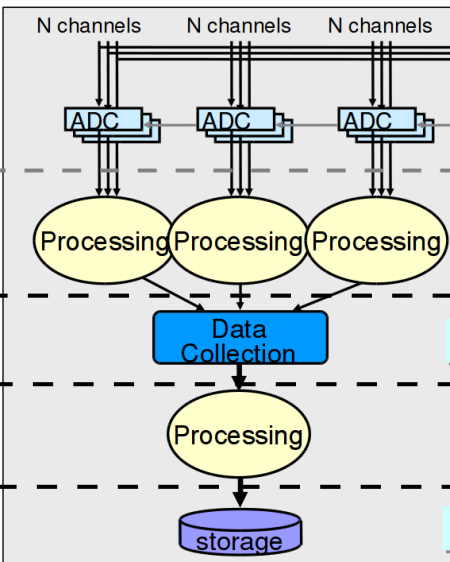
\includegraphics[scale=0.3]{./images/daq.png}
    \caption{}
    \label{fig:}
  \end{center}
\end{figure}

\subsection{Reconstruction and calibration}
What is measured in ALICE and its detectors are electrical signals. These signals have to be reconstructed in order to conclude that a particle has been present. The reconstruction has to take the detector conditions into account. This calibration is currently been done offline but will be done both offline as an asynchronous process and online as a synchronous process in the future. When the calibration is done online downtime of the computers working on the calibration will result in data loss. Because the calibration will be an integral part of the online system and each delay in this system will have immediate repercussions further up the line.

On the same original raw data set multiple reconstruction passes can be done. This can be due to having found a bug in earlier reconstruction software and better software is developed or finding a not yet detected bias in the raw data resulting in a better calibration set. A new calibration set now becomes available within months. In the future this could be within hours. And so the system should be very flexible. It may happen that the same data will be re-calibrated 20 times. With the help of metadata this must be book kept.

The Light Production Management runs operations on the offline activities which are done on the Grid. In Figure \ref{fig:offlineWorkflow} the CPasses are dry runs and OAD are Object Analysis Data. Such offline activity is done 24 hours each day of the week and all year along.


\subsection{Simulation}
To know which collisions are of interest and what we can learn from these collisions, simulations are created using among other methods the Monte Carlo (MC) statistical method. These simulations are run on the Grid and are completely decoupled from LHC operations. Normally such simulations are associated with or anchored to an actual raw data set taken from a run, i.e. the conditions for the run are the same as for the simulations. There is no limit to the number of MC productions for a particular run. A new MC production can be started because of better software becoming available or because the chosen parameters are different.


\subsection{Data Preparation Group}
Data Preparation Group was created for to do:
\begin{itemize}
  \item data preparation, i.e. reconstruction and simulation. This consists of production configuration, setup, calibration monitoring.
  \item data processing, i.e. monitoring, execution, reporting, bug tracking.
  \item quality assurance, i.e. validation and creating lists of good runs or data sets.
\end{itemize}




\subsection{Analysis}
Physicists from all over the world are doing analyses on the reconstructed data and produce papers about their findings. The physicists are the end user of ALICE and the bookkeeping system. The analyses are run on the Grid which is completely decoupled from the LHC operations. Normally these analyses run as trains, i.e. multiple analysis jobs using the same data sets are packed together.



\section{The ALICE upgrade}
During the Long Shutdown 2 ALICE will be upgraded. The upgrade will be done on many subsystems:
\begin{description}
  \item[ITS] A new Inner Tracking System will be installed. This new system will have an improved pointing precision. It will also be made of lesser material than before and become the thinnest tracker at the LHC.
  \item[TPC] The Time Projection Chamber will get new GEM technology for the read out chambers. The readout will be continuous and it will use faster readout electronics.
  \item[CTP] A new Central Trigger Processor will be installed.
  \item[DAQ] A brand new Data Acquisition system will be installed.
  \item[HLT] A new High Level Trigger will be installed.
  \item[MFT] In the Muon Forward Tracker a new SI tracker will be installed. The MUON pointing precision will be improved.
  \item[MUON ARM] The MUON ARM will get new continuous readout electronics.
  \item[FIT] There will be new Trigger detectors installed.
  \item[TOF] The TOF will be readout faster.
  \item[TRD] The TRD will be readout faster.
  \item[ZDC] The ZDC will be readout faster.
\end{description}

\begin{figure}[h]
  \begin{center}
    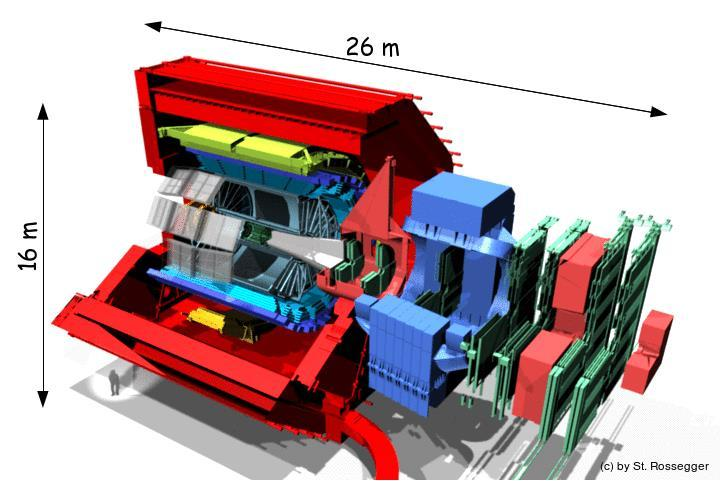
\includegraphics[scale=0.4]{./images/alice_upgrade.jpg}
    \caption{An overview of ALICE}
    \label{fig:overview}
  \end{center}
\end{figure}
After the Long Shutdown 2 the LHC produce Pb–Pb collisions at up to $L = 6.10^{27} cm^{-2} s^{-1}$. This results in an interaction rate of 50kHz. During Run 3 (2021-2023) pp collisions will be done at 14 TeV and Pb-Pb collisions at 5.5 TeV. In 2023 no Pb-Pb collisions are scheduled. After Long Shutdown 3 (2024-2026) the same schedule will be realised except for 2028 when p-Pb will be run at 8.8 TeV.

The 50 kHz rate for collisions produces about 100 times more data than was produced in 2010. This will give the physicists the opportunity to detect very rare processes with very small signal over background ratio. Because the triggering techniques are very inefficient if not impossible support for continuous read-out is developed. Therefore a new computing system, $O^2$, is created. It will read-out the data of all interactions. Compress these data intelligently by online reconstruction. The system will be one common online-offline computing system.

Unmodified raw data of all interactions shipped from detector to online farm in triggerless continuous mode. This will amount to 3.4 TB/s. Then a baseline correction and zero suppression will take place. The data volume will be reduced by zero cluster finder. No event is discarded. The average compression factor is 6.6. Then 500 GB/s will be shipped. A data volume reduction is done by online tracking. Only reconstructed data will be send to data storage. The average compression factor is 5.5. From here 90 GB/s will be transported. In the data Storage 1 year of compressed data will be kept. From this storage facility 20 GB/s will be transported to tier 0 and tier 1. The events will also be reconstructed for final calibration.

From the detector electronics 8500 GBTs links will send signals to the 270 FLPs. These will use hardware acceleration using FPGAs. A switching network will distribute this data to 1500 EPNs. These processing nodes use GPUs for hardware acceleration. The EPNs use a switching network to send the data to the storage. This storage can write at 170 GB/s and read at 270 GB/s. The capacity for storage is 60 PB.

To manage the $O^2$ update several work packages are created:
\begin{description}
  \item[WP 1] Data Model
  \item[WP 2] Data Flow and System Simulation
  \item[WP 3] Common Tools and Software
  \item[WP 4] $O^2$ Software Framework– Common tools and infrastructure
  \item[WP 5] Data distribution and load balancing
  \item[WP 6] Detector readout
  \item[WP 7] Quality Control
  \item[WP 8] Control, Configuration and Monitoring
  \item[WP 9] Event Display
  \item[WP 10] Constant and Calibration DB
  \item[WP 11] ALFA
  \item[WP 12] Simulation
  \item[WP 13] Reconstruction and Calibration
  \item[WP 14] Analysis framework and facility infrastructure
  \item[WP 15] Data Management
  \item[WP 16] Computing Room CR1 (FLP)
  \item[WP 17] Computing Room CR0 (EPN)
\end{description}

\section{Purpose}
The purpose of this Software Requirements Specifications document is to have a central point for all the requirements of the bookkeeping system. It is not written with the goal to have a document with definite and final requirements for this system. During the process of developing this system requirements will be added and modified.

\subsection{Upgrade of the bookkeeping}
ALICE will do a major upgrade in 2019/2020 when the Long Shutdown 2 will be done. During this period the new Online-Offline ($O^2$) computer system will be implemented. This gives an opportunity to upgrade the bookkeeping facility currently in use. The bookkeeping currently consists of two not related systems: the Electronic Logbook and AliMonitor. These systems have been developed since 2009 and evolved gradually during the years. Due to this development process the applications are in some ways a bit confusing, not efficient and overall candidates for improvement, let alone their fusion which seems an improvement in itself. In Section XX a description of the current system is given. It seems to be most sensible to do such an during a Long Shutdown because of the overall break in activities at ALICE. New detectors are being installed, the LHC stops running, etc. An update done during a winter break which is always taking place between half December and March would have been a possibility. Doing such an update during run season does not seem to be appropriate because of the importance of the bookkeeping system for ALICE. It is expected that the next opportunity to replace the current systems is over 10 years. That would take too long for the current systems to exist.

\begin{figure}[h]
  \begin{center}
    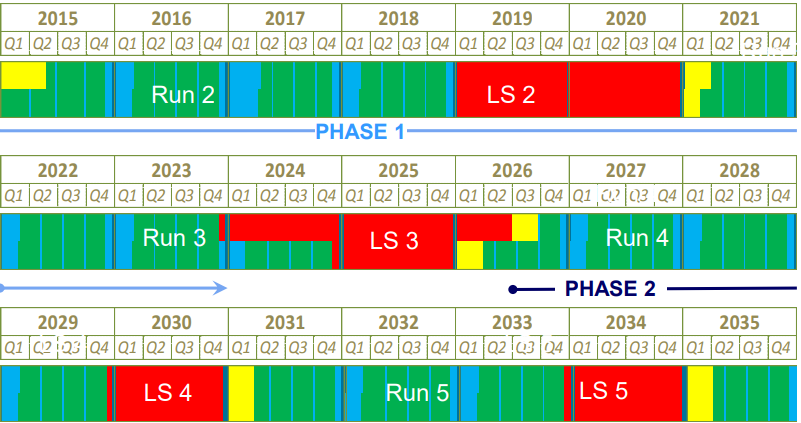
\includegraphics[scale=0.3]{./images/timetable.png}
    \caption{Time table for the LHC}
    \label{fig:timetable}
  \end{center}
\end{figure}

The motivation to do an upgrade is threefold. First it makes sense to unify the two systems, i.e. the electronic logbook and AliMonitor, now used to bookkeeping for ALICE. In this respect it should be mentioned that some users of AliMonitor themselves use separate systems to store information which arguably should be part of the bookkeeping system, e.g. JIRA. Secondly, although in the years of its existing a lot of features were added, this is not been done anymore since it was clear the system would be replaced. Features which have been mentioned the last few years are only when really needed, implemented. This means that there is a list of features not implemented but still wished for. Lastly, because the system was developed starting around 2009 it is based on relatively old technologies. 

The goal is a bookkeeping system which is responsive to different media used and has a unified look and feel. It should be compatible to the current system and accessible from inside and outside of CERN. The authorisation and authentification should be based on the central systems as made available by CERN. It should be supported as long as it is in use by ALICE.

There are several challenges for the update of the bookkeeping system. The bookkeeping system is critical to the ALICE operations. It is critical because without proper bookkeeping of the data, i.e. bookkeeping the metadata referring to the physics data produced by ALICE, the data itself, i.e. the data produced by the detectors, becomes useless. The workflows which should be registered in the system are quite complex. Because the AUAS is a newcomer to the High Energy Physics community a lot has to be learned about vocabulary and jargon. The schedule for the project is also a challenge. At the end of next year (2018) a (small) part of the system has to be delivered while the whole system should be in production in 2021. Another difficulty for the project is found in the migration from the existing to the new tool. A part of the bookkeeping system concerns the off line activity for recovering data and quality control. This work will not stop during the Long Shutdown 2 and for this work to be done a continuous use of the system will take place. Lastly, support for the system will have to be done until 2029.

During Run 1 and 2 a lot of experience concerning the use of the bookkeeping system is accumulated. Developers of the new system have the opportunity to elicit the experience of the past users and use this to their advantage. Modern technologies should make it more easy to develop a bookkeeping system. Because the AUAS is the task owner to create the bookkeeping system it is expected this should generate a lot of energy to make it happen.

\subsection{Vision}
Provide unified bookkeeping experience for operations, run catalogue and management.

\subsection{Needs}
Access in a single place all metadata related with operational activities. Keep historical record of used configurations, statistics and data quality. Produce reports for operational teams and management. 

\subsection{Product}
Dashboards for run metadata with different levels of detail. Search for data sets that match given criteria. Forms for creating textual log entries. Notifications for interventions, main events and summary reports. API for read/write access to metadata repository. 


\subsection{Business goals}
Adapt to new O2 data model. Consolidate existing ALICE Electronic Logbook and Run Conditions Table in a single product. Refresh used technologies and make the product more future oriented. Integrate gathered experience and introduce missing features. 



\section{Scope of the Bookkeeping System}
The scope of the project to develop the bookkeeping system is restricted to keeping track of the configuration of ALICE, data produced by ALICE, and computations on this data. The bookkeeping system is not a monitoring system for ALICE.


\subsection{Overview of the current bookkeeping}

The bookkeeping is important because of several reasons. In the bookkeeping system accounting is done for:
\begin{itemize}
  \item configurations of the detectors during the data taking runs,
  \item the conditions which existed during the data taking runs,
  \item the statistics which are generated using the data.
\end{itemize}

The bookkeeping system is also used to search and select specific data concerning these runs. Questions such as `which runs included detector X?' or `which data sets should I use for my analysis?'. Furthermore, it is used for manually and automaticaly generating data about for instance how much data was collected during a given period or the efficiency during a period.

Momentarily there are two systems which are part of the bookkeeping system:
\begin{itemize}
  \item the electronic logbook (http://cern.ch/alice-logbook),
  \item AliMonitor (http://alimonitor.cern.ch/).
\end{itemize}
A few scattered repositories are also used. These are mainly human-curated web pages.


\subsubsection{The electronic logbook}
The logbook is gathering data in synchronous mode i.e. synchronous with the LHC operations. These log entries are created by:
\begin{itemize}
  \item run coordinator (and deputy), shift leader and shifters which are 24/7 present when data is taken in.
  \item technical coordination, for cooling etc.
  \item detector teams for expert interventions (during on call interventions)
  \item automatically by elements of the machine.
\end{itemize}

In the logbook are online configurations and statistics of the:
\begin{itemize}
  \item Data Acquisition system (DAQ),
  \item High Level Trigger (HLT),
  \item Trigger,
  \item Large Hydron Collider (LHC),
  \item Detector Monitoring Systems (TPC etc.),
  \item runs where the runnumber is always a positive integer,
  \item LHC fills.
\end{itemize}

In all the logbook has approximately
\begin{itemize}
  \item 37 GB data,
  \item 195,000 log entries,
  \item 20,000 file attachments,
  \item 280,000 runs
  \item 5,000 LHC fills
\end{itemize} 37 GB data, 195

For this it uses a MySQL database with 27 tables and 312 fields. This is a single instance which is daily copied for external uses. Back-ups are sent to CERN-IT. The logbook has several APIs:
\begin{itemize}
  \item C for core software,
  \item DIM for detector teams,
  \item REST for other systems.
\end{itemize}
The Web GUI is created by using PHP on the server side. For this no framework is used. On the client side Javascript is used.


\subsubsection{AliMonitor}

The AliMonitor is for bookkeeping of the Grid operations done to process data with the goal discerning data usable for (specific) physics analysis and data which is not. The AliMonitor is operating in an asynchronous mode, i.e. asynchronous with the LHC operations.The Grid is composed of Tier 0 and Tier 1 computers located at CERN and Budapest (Tier 0) and at 10 other places around the world (such as SARA and Nikhef (Amsterdam) for Tier 1. Users of AliMonitor are:
\begin{itemize}
  \item Data Preparation Group (DPG) to do reconstruction and simulation,
  \item Physics Working Groups for simulation and analysis
  \item ALICE physicists for simulation and analysis.
\end{itemize}
The activities done on the Grid are called jobs. A masterjob is loosely coupled on a run. Each masterjob is composed of subjobs which are loosely coupled on raw files.These jobs can be reconstruction passes and Monte Carlo (MC) productions. Reconstruction is done to adjust the data and get rid of biasses always present due to imperfection of the detectors. For example, it is known that the TPC for muons a bias of 5 microns creates. This is being corrected during reconstruction. Although a lot of these jobs are automated human intervention is possible.

The calibration and correction of raw data is not a one time event but can be done several times because of several reasons. It is possible that it is discovered that there is a specific bias in the data which should be corrected. It is possible someone creates a better algorithm, etc. The re-calibration is now being done within months. In the future it might be possible it will be done within hours because a part of the reconstruction will be done online. Because it is possible that data will be re-calibrated maybe even as often as 20 time the new bookkeeping system should be so flexible it can handle various scenarios.

When different jobs are being done on the same data so called trains are made. These trains are wagons of jobs which process all the same data. From the viewpoint of efficiency this makes a lot of sense. The LPM initiates this sort of operations.

In all there is 97 GB data. There are 12.9 million master jobs (1 million simulation, 225,000 reconstruction, 5 million organised analysis and 6.5 million user jobs). There are 1 billion subjobs which are not stored permanently but summarized per master job. In the LPM there are 56,000 processing chains which are grouped in 13,000 job types (aka productions).

AliMonitor is using a PostgreSQL database with about 30 tables. It has two instances which are periodically back-upped. There are APIs for JDBC to be used for core processes and HTTP for csv- and XML-files. The web GUI is realised by a Tomcat webserver using Java Server Pages.

\subsubsection{Scattered repositories}
There are a few scattered repositories such as:
\begin{itemize}
  \item twiki
  \item Jira
  
\end{itemize}



The bookkeeping system consists of two distinct subsystems with separate features and deadlines:
\begin{itemize}
  \item At 1 January 2019 the electronic logbook feature of the bookkeeping system has to be in place to be of assistance for the commissioning of several subsystems. 
  \item the $O^2$ software has to be in place later. This concerns functionalities such as:
  \begin{itemize}
    \item datataking
    \item QA
    \item log activities
    \item statistics for runs
    \item database, for which a bookkeeping model is needed. This defined by what we want to store.
  \end{itemize}
  \item GUI
  \item reporting
\end{itemize}
In the middle of 2020 a global commission is planned. Than a synchronous reconstruction should be possible. The generation of reports should be possible starting January 2021. Then a clean start with the system will be made.

\begin{tabular}{cc}
\hline
Feature & deadline\\
\hline
\hline
 Reconstruction and callibration  & 2020 commissioning \\
 \hline
Simulation   & 2020\\
\hline
Analysis & 2020\\
\hline
\end{tabular}

\subsection{Migration}
Data taking with the current system stops end 2018. Then a migration can be done. Old statistics from the current system should be combined with the new system. And the data stored in the old database should be migrated to the new database. Or the old database could be kept in place and have an interface with the new system. 

The offline activities will be going on. A date has to be set to use the new bookkeeping system. It should be carefully prepared which part will be migrated.

Collaborative tools will be used. The bookkeeping system is part of WP 8. WP 8 has once every two weeks a meeting at Tuesday morning at 10.00 AM. Once every two months the $O^2$ technical board meets. 

An $O^@$ data model for bookkeeping should be available in January 2018.



\section{Definitions, Acronyms, and Abbreviations}




\subsection{Log Entry}
A Log Entry is a text message that describe an intervention or an event that happened. It can be generated either by humans (e.g. a shifter enters his/her end-of-shift report) or by machines (e.g. a detector logs some abnormal situation automatically). 

\subsection{Run}
A Run is a unique ID that identifies a synchronous data processing session in the $O^2$ computing system with a specific and well-defined configuration. It normally ranges from a few minutes to tens of hours. It is generated and managed by the $O^2$ system. 

\subsection{LHC Fill}
An LHC Fill is a unique ID that identifies a period of activity in the LHC accelerator. It normally ranges from a few minutes to tens of hours. It is generated and managed by the LHC system and published via DIP protocol. 

\subsection{Offline metadata model}
The offline activities are administered by AliMonitor\footnote{Most information provided in this chapter is gathered during an interview with Costin Grigoras on Tuesday 12 December 2017}. Costin Grigoras is the main developer of this system. The current system is the minimum which is needed for this activity. Figure \ref{fig:offlineWorkflow} shows the workflow off the offline activities. Castor is software to manage tapes on CERN tier 0. For all these files there is an url stored in ALien (e.g. pointers). Shuttle is calibration data stored on EOS. The Lightweight Production Manager (LPM) is software to manage disks on CERN. The LPM decides based on several variables that a run will be reconstructed. CPass means Calibration Pass. 

\begin{figure}
  \begin{center}
    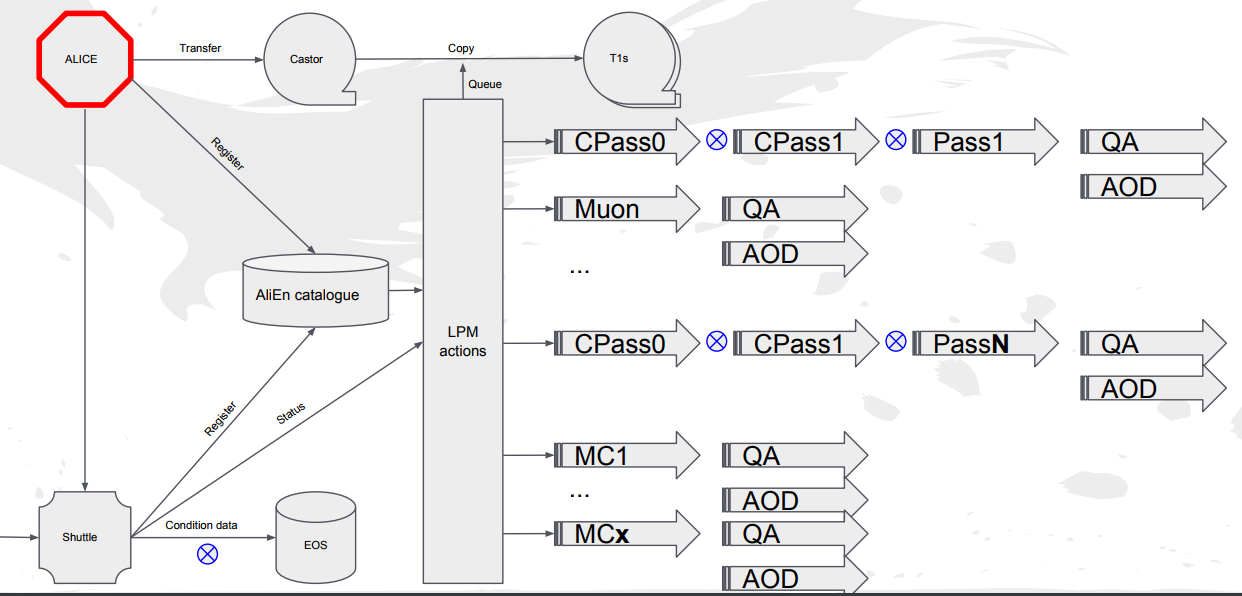
\includegraphics[scale=0.25]{./images/offline_workflow.png}
    \caption{Calibrating and reconstructing the signals}
    \label{fig:offlineWorkflow}
  \end{center}
\end{figure}

\subsubsection{Run entity}
Run entities are in several forms. There is the period name (an integer and alphanumeric letter). When conditions are simular the period name is kept. This may take weeks. So there are 10 to 15 periods each year. Run change very often. A period name is a short cut for same sort of runs.
\begin{figure}
  \begin{center}
    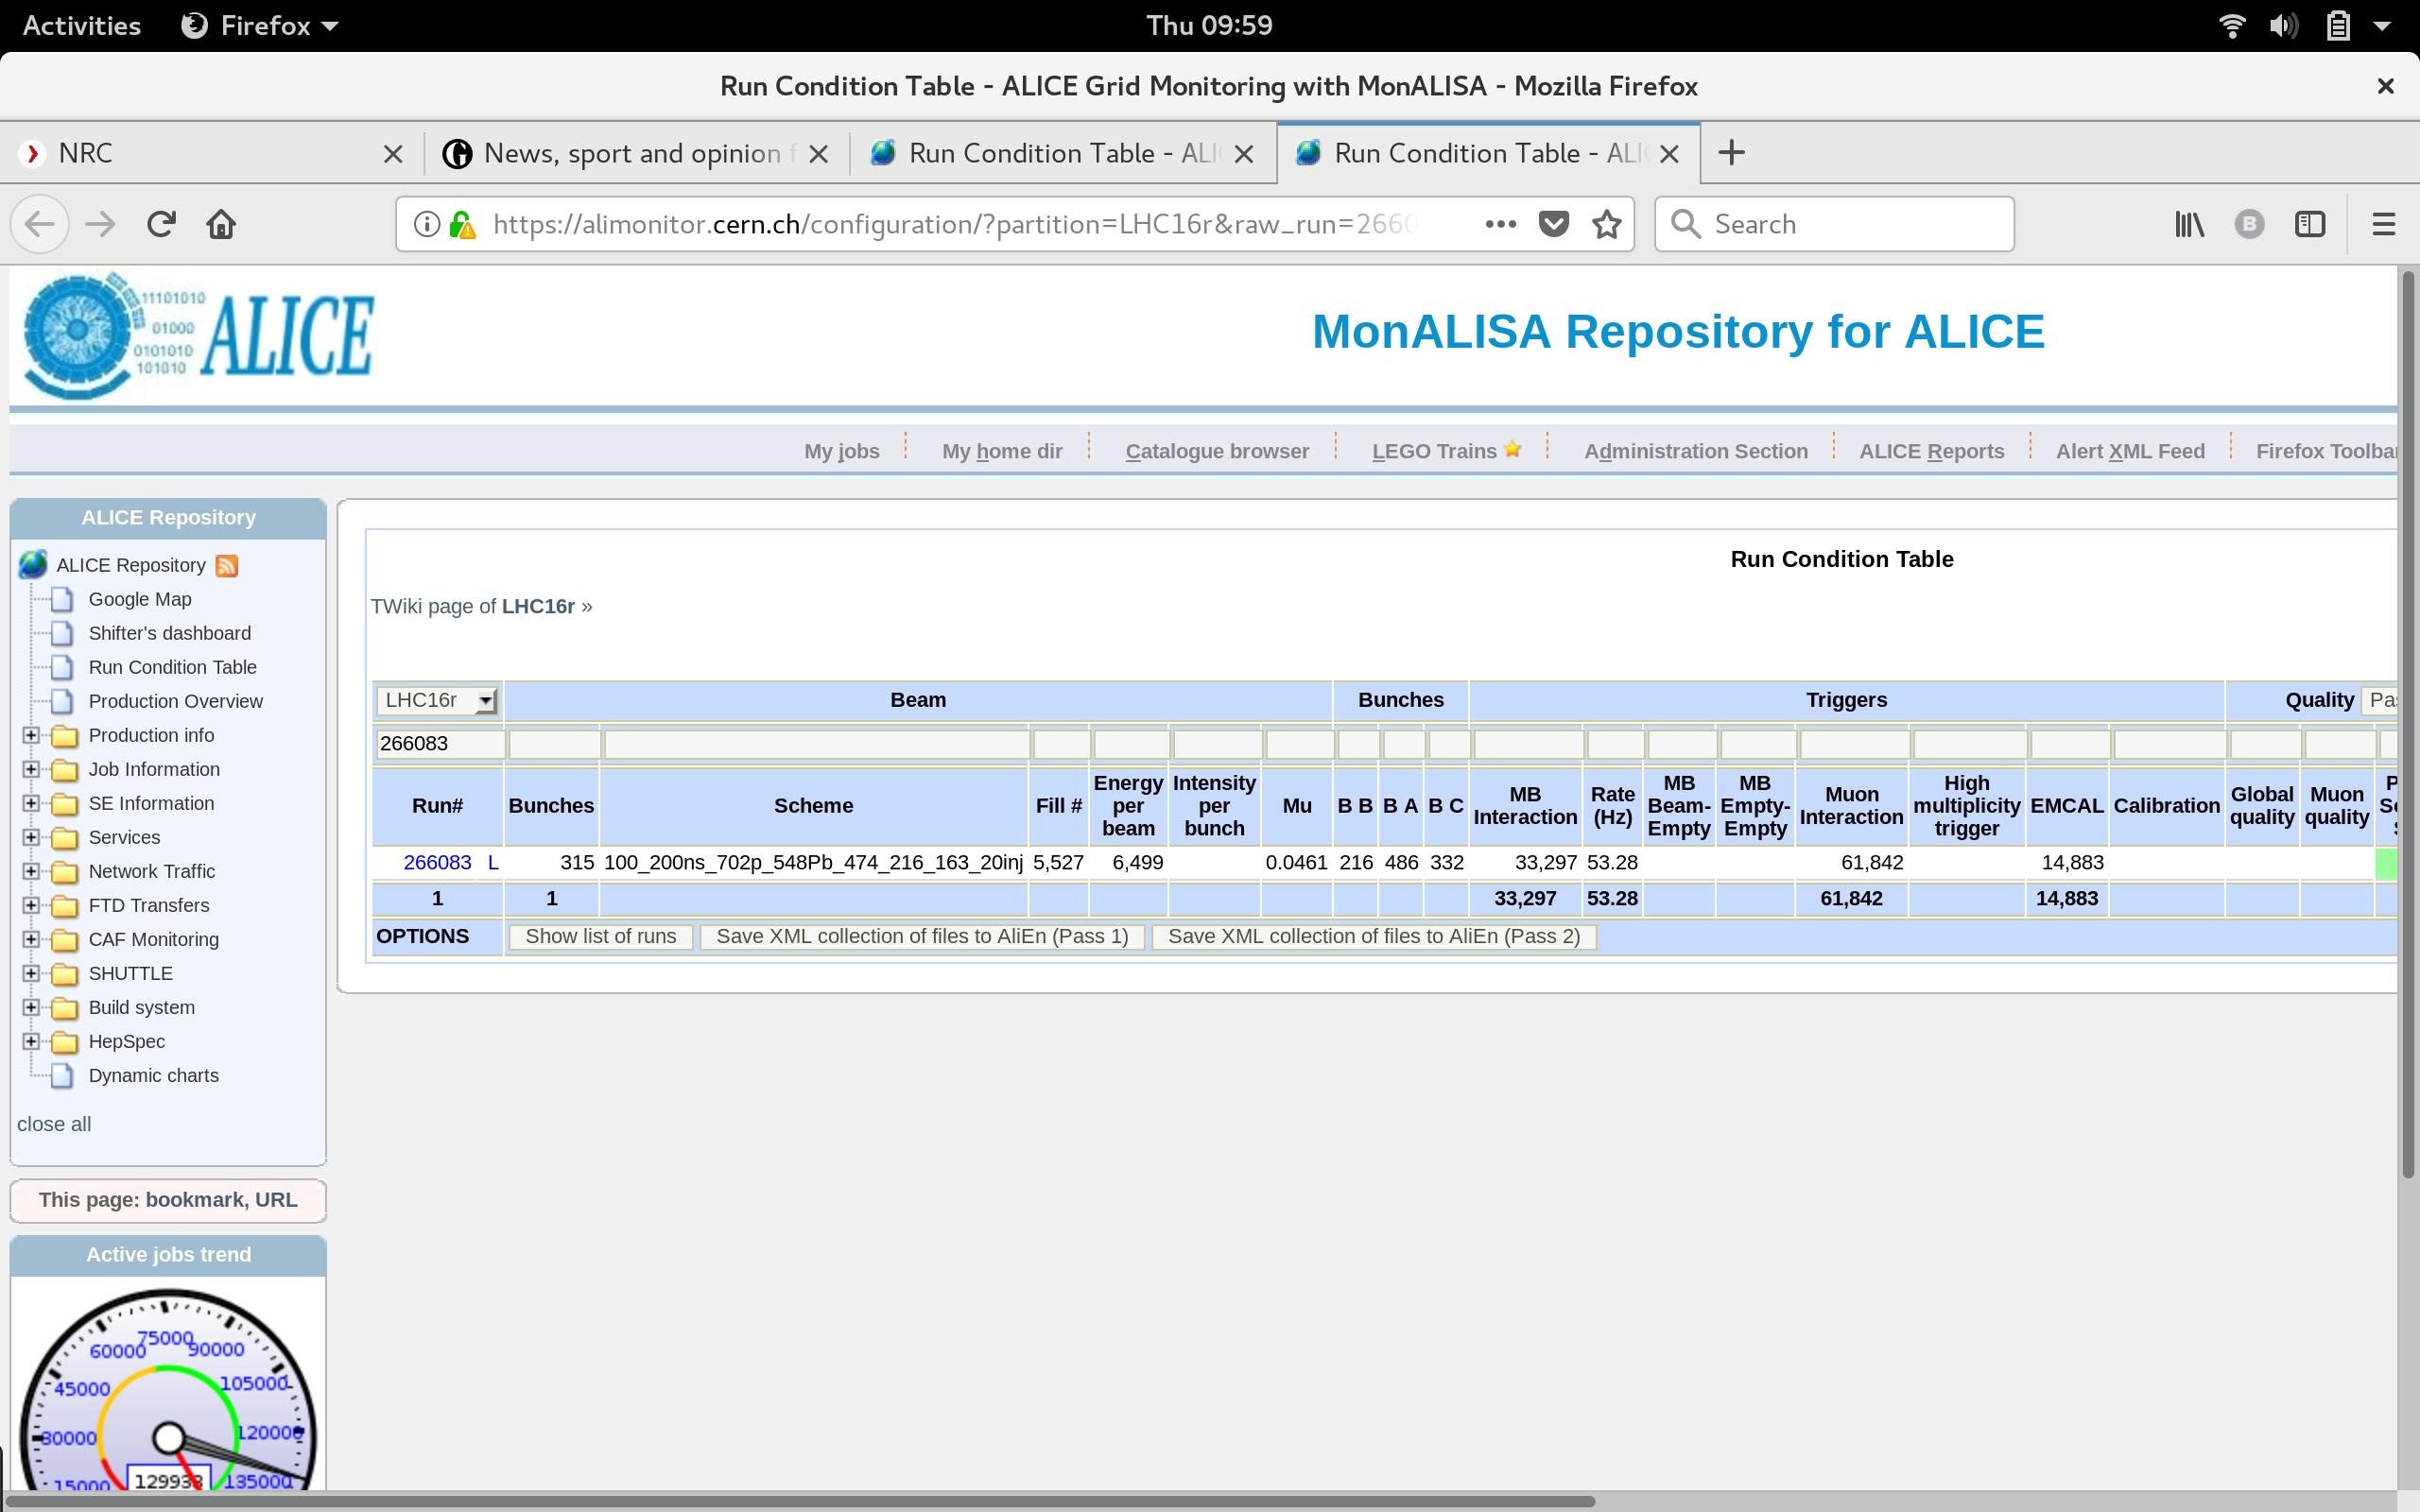
\includegraphics[scale=0.15]{./images/run_entity.png}
    \caption{Screenshot of run condition table}
    \label{fig:run_con_table}
  \end{center}
\end{figure}

In Figure \ref{fig:run_con_table} a screenshot of the run condition table is shown. In here the period name and interaction type can be found. The number of raw data chunks and the total size. Also the AliEn directory where the data is located. The specific detectors which participated in this run and the SHUTTLE-status. At last one can find the number of events in several classes.

\begin{figure}
  \begin{center}
    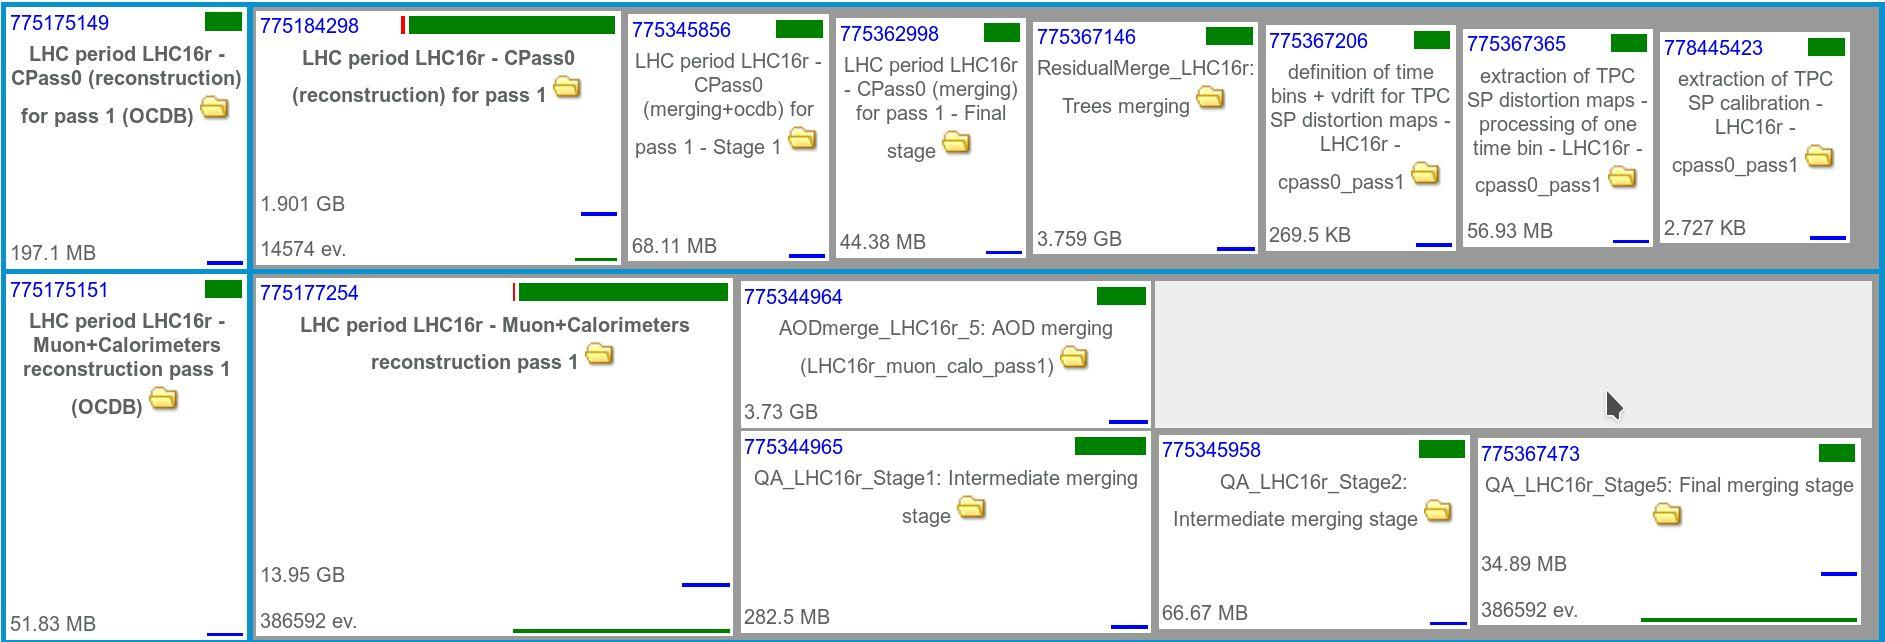
\includegraphics[scale=0.2]{./images/run_view.jpg}
    \caption{A run view}
    \label{fig:run_view}
  \end{center}
\end{figure}


\begin{figure}
  \begin{center}
    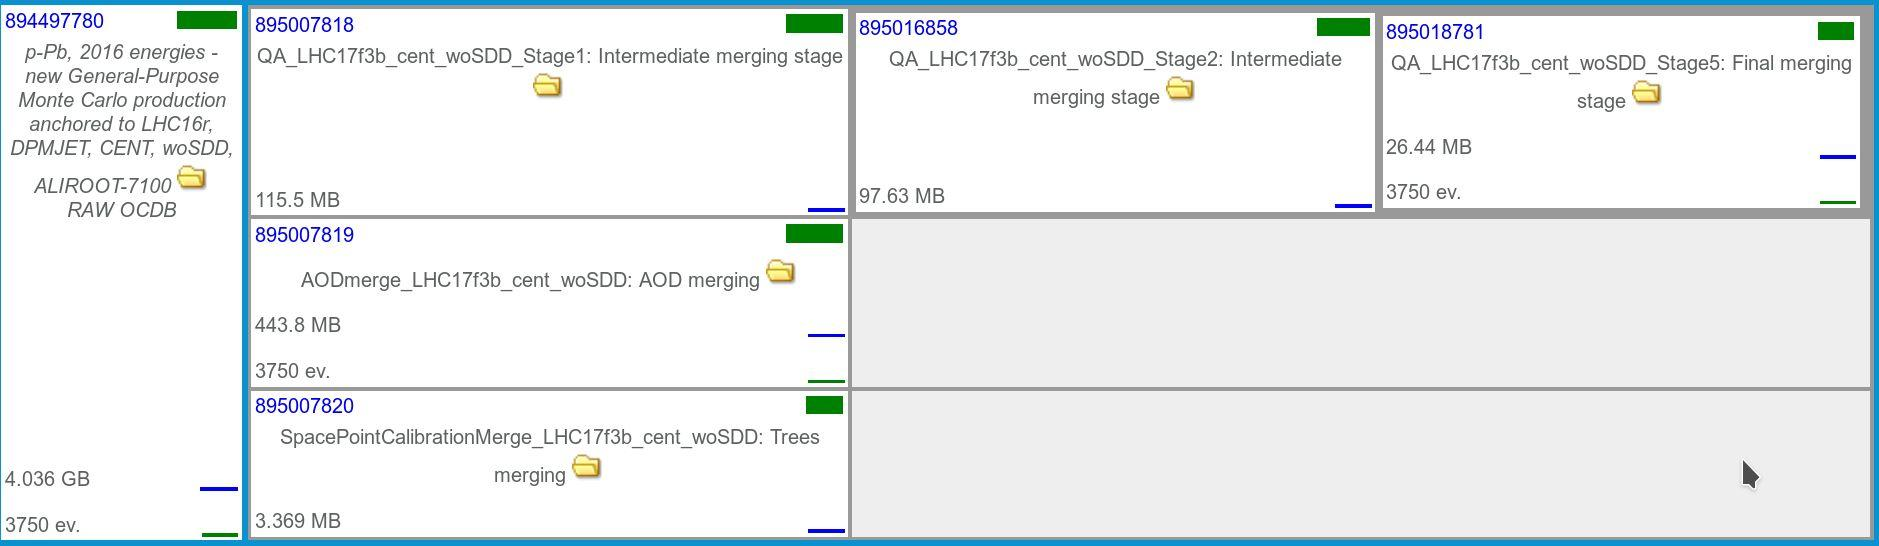
\includegraphics[scale=0.2]{./images/run_view_mc.jpg}
    \caption{A Monte Carlo run view}
    \label{fig:run_view_mc}
  \end{center}
\end{figure}

The coding scheme is human made. In the run view a masterjob ID is shown on the upper left side. This identifier is unique. A masterjob can be divided into subjobs per file. A Monte Carlo view is more or less the same. Such a run can be based on the conditions a raw file is produced. In such a case it is called anchored to a raw file. On the upper right side a color code indicates the status of the (sub-) job. The firs process for each file is a snapshot of the raw data in order to determine the same conditions for every process.

The software version for each period(name) is the same. This is not hard. Software versions don't change during a run. The data self should never be transferred. Always a pointer to a file is used. The configuration data can be transferred. When a masterjob is done then statistics are generated. 

\begin{figure}
  \begin{center}
    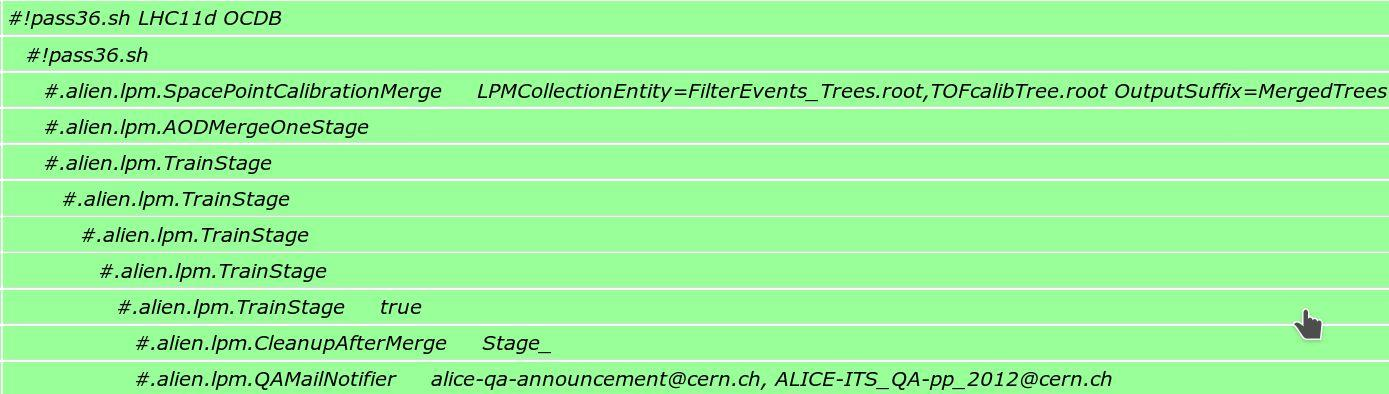
\includegraphics[scale=0.25]{./images/workflow.jpg}
    \caption{}
    \label{fig:}
  \end{center}
\end{figure}

The workflow has many steps:
\begin{itemize}
  \item OCDB snapshot creation (single special job)
  \item Per chunk reconstruction (one subjob per chunk)
  \item TPC SpacePointCalibration
  \item AOD merging (many chunk AODs to one file)
  \item QA merging in stages (to get a single QA\_results.root file per run)
  \item Sending notification emails / cleanup of intermediate steps
\end{itemize}

Pass 36 is just a name. 

\begin{figure}
  \begin{center}
    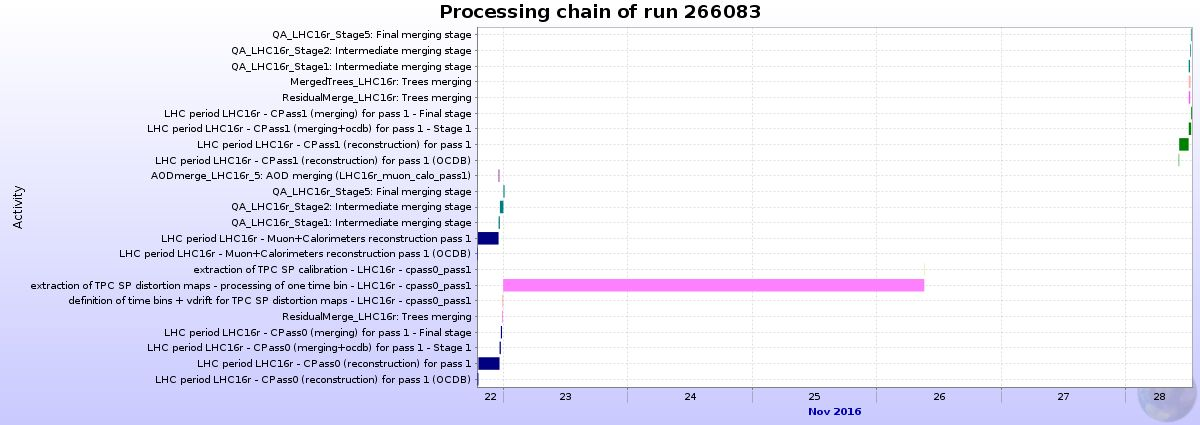
\includegraphics[scale=0.25]{./images/timeline.png}
    \caption{A timeline of a run}
    \label{fig:timeline}
  \end{center}
\end{figure}

A timeline such as shown in Figure \ref{fig:timeline} is needed.

\subsection{metadata structures}
\subsubsection{Production}
All (master) jobs of a given type are grouped together. They get a unique tag, eg. LHC17g8a\_fast. Here is `17' the year of production, `g' a symbol for Monte Carlo jobs and `8a' a number given by the bookkeeping system. A common description of characteristics of the data and software packages used is:
\begin{quotation}
p-Pb, 5.02 TeV - JJ events embedded in EPOS-LHC events anchored to LHC16qt, FAST only, ALIROOT-7270
\end{quotation}
The type of masterjob can be:
\begin{itemize}
  \item MC,
  \item RAW, 
  \item Merging, 
  \item Filtering, 
  \item Train, 
  \item ... (something else in the future).
\end{itemize}
Part of this administration is also the requested or produced number of events. Also, it should be administered when was the last time a period or run was accessed.

\subsubsection{Job}

A job is a wrapper around an AliEn masterjob ID. It belongs to a production ID. There is an owner and an output directory. The parent job ID should also be given to chain processes. The accounting information to register is:
\begin{itemize}
  \item Output size, analyzed/produced events
  \item CPU, Wall time, i.e. how long a job stayed on a worker node (this should be a bit longer than CPU time)
  \item No. of subjobs in each state
  \item Submission/completion timestamp
  \item Stack traces for failed jobs
\end{itemize}


\begin{figure}
  \begin{center}
    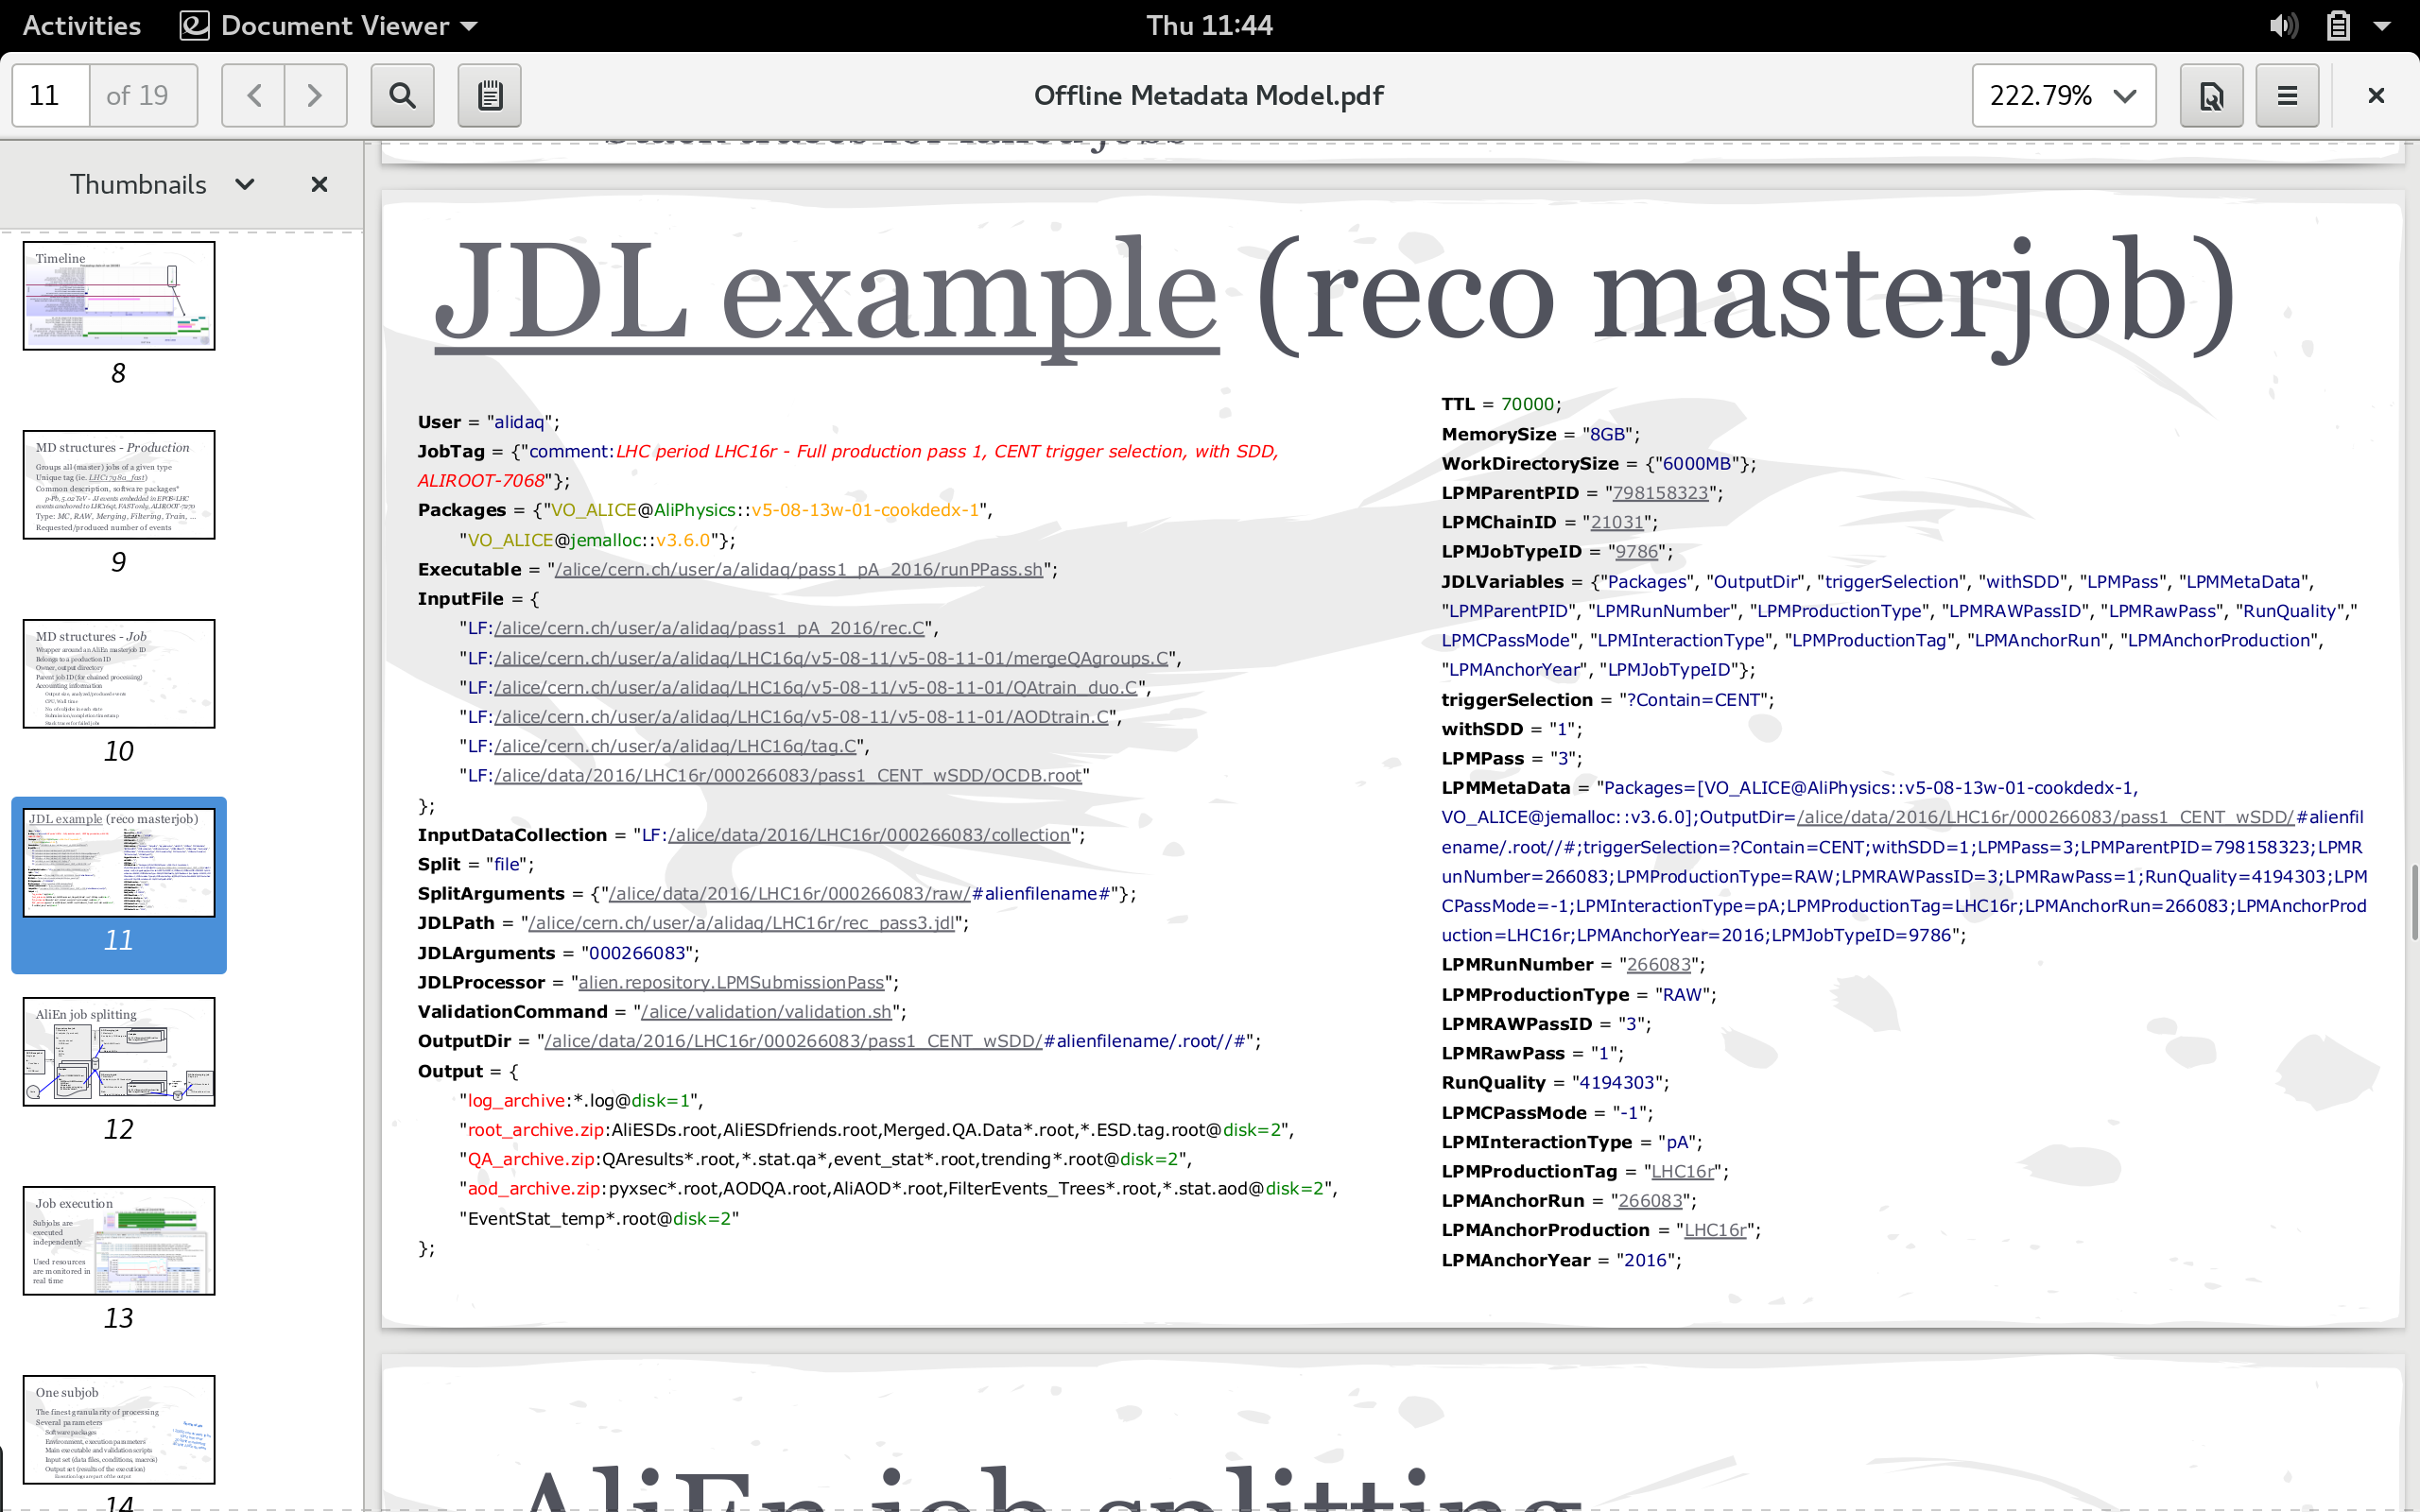
\includegraphics[scale=0.15]{./images/jdl_example.png}
    \caption{An example of a JDL reconstruction masterjob}
    \label{fig:jdl_example}
  \end{center}
\end{figure}
Figure \ref{fig:jdl_example} shows an example of a reconstruction masterjob written in Job Description Language (JDL). Event Summary Data (ESD) should be generated. The job execution is stored for a week. Some statistics concerning these activities would be nice to have.

\subsubsection{Subjobs}
Jobs can be split into subjobs as shown in Figure \ref{fig:splitting_subjobs}.

\begin{figure}
  \begin{center}
    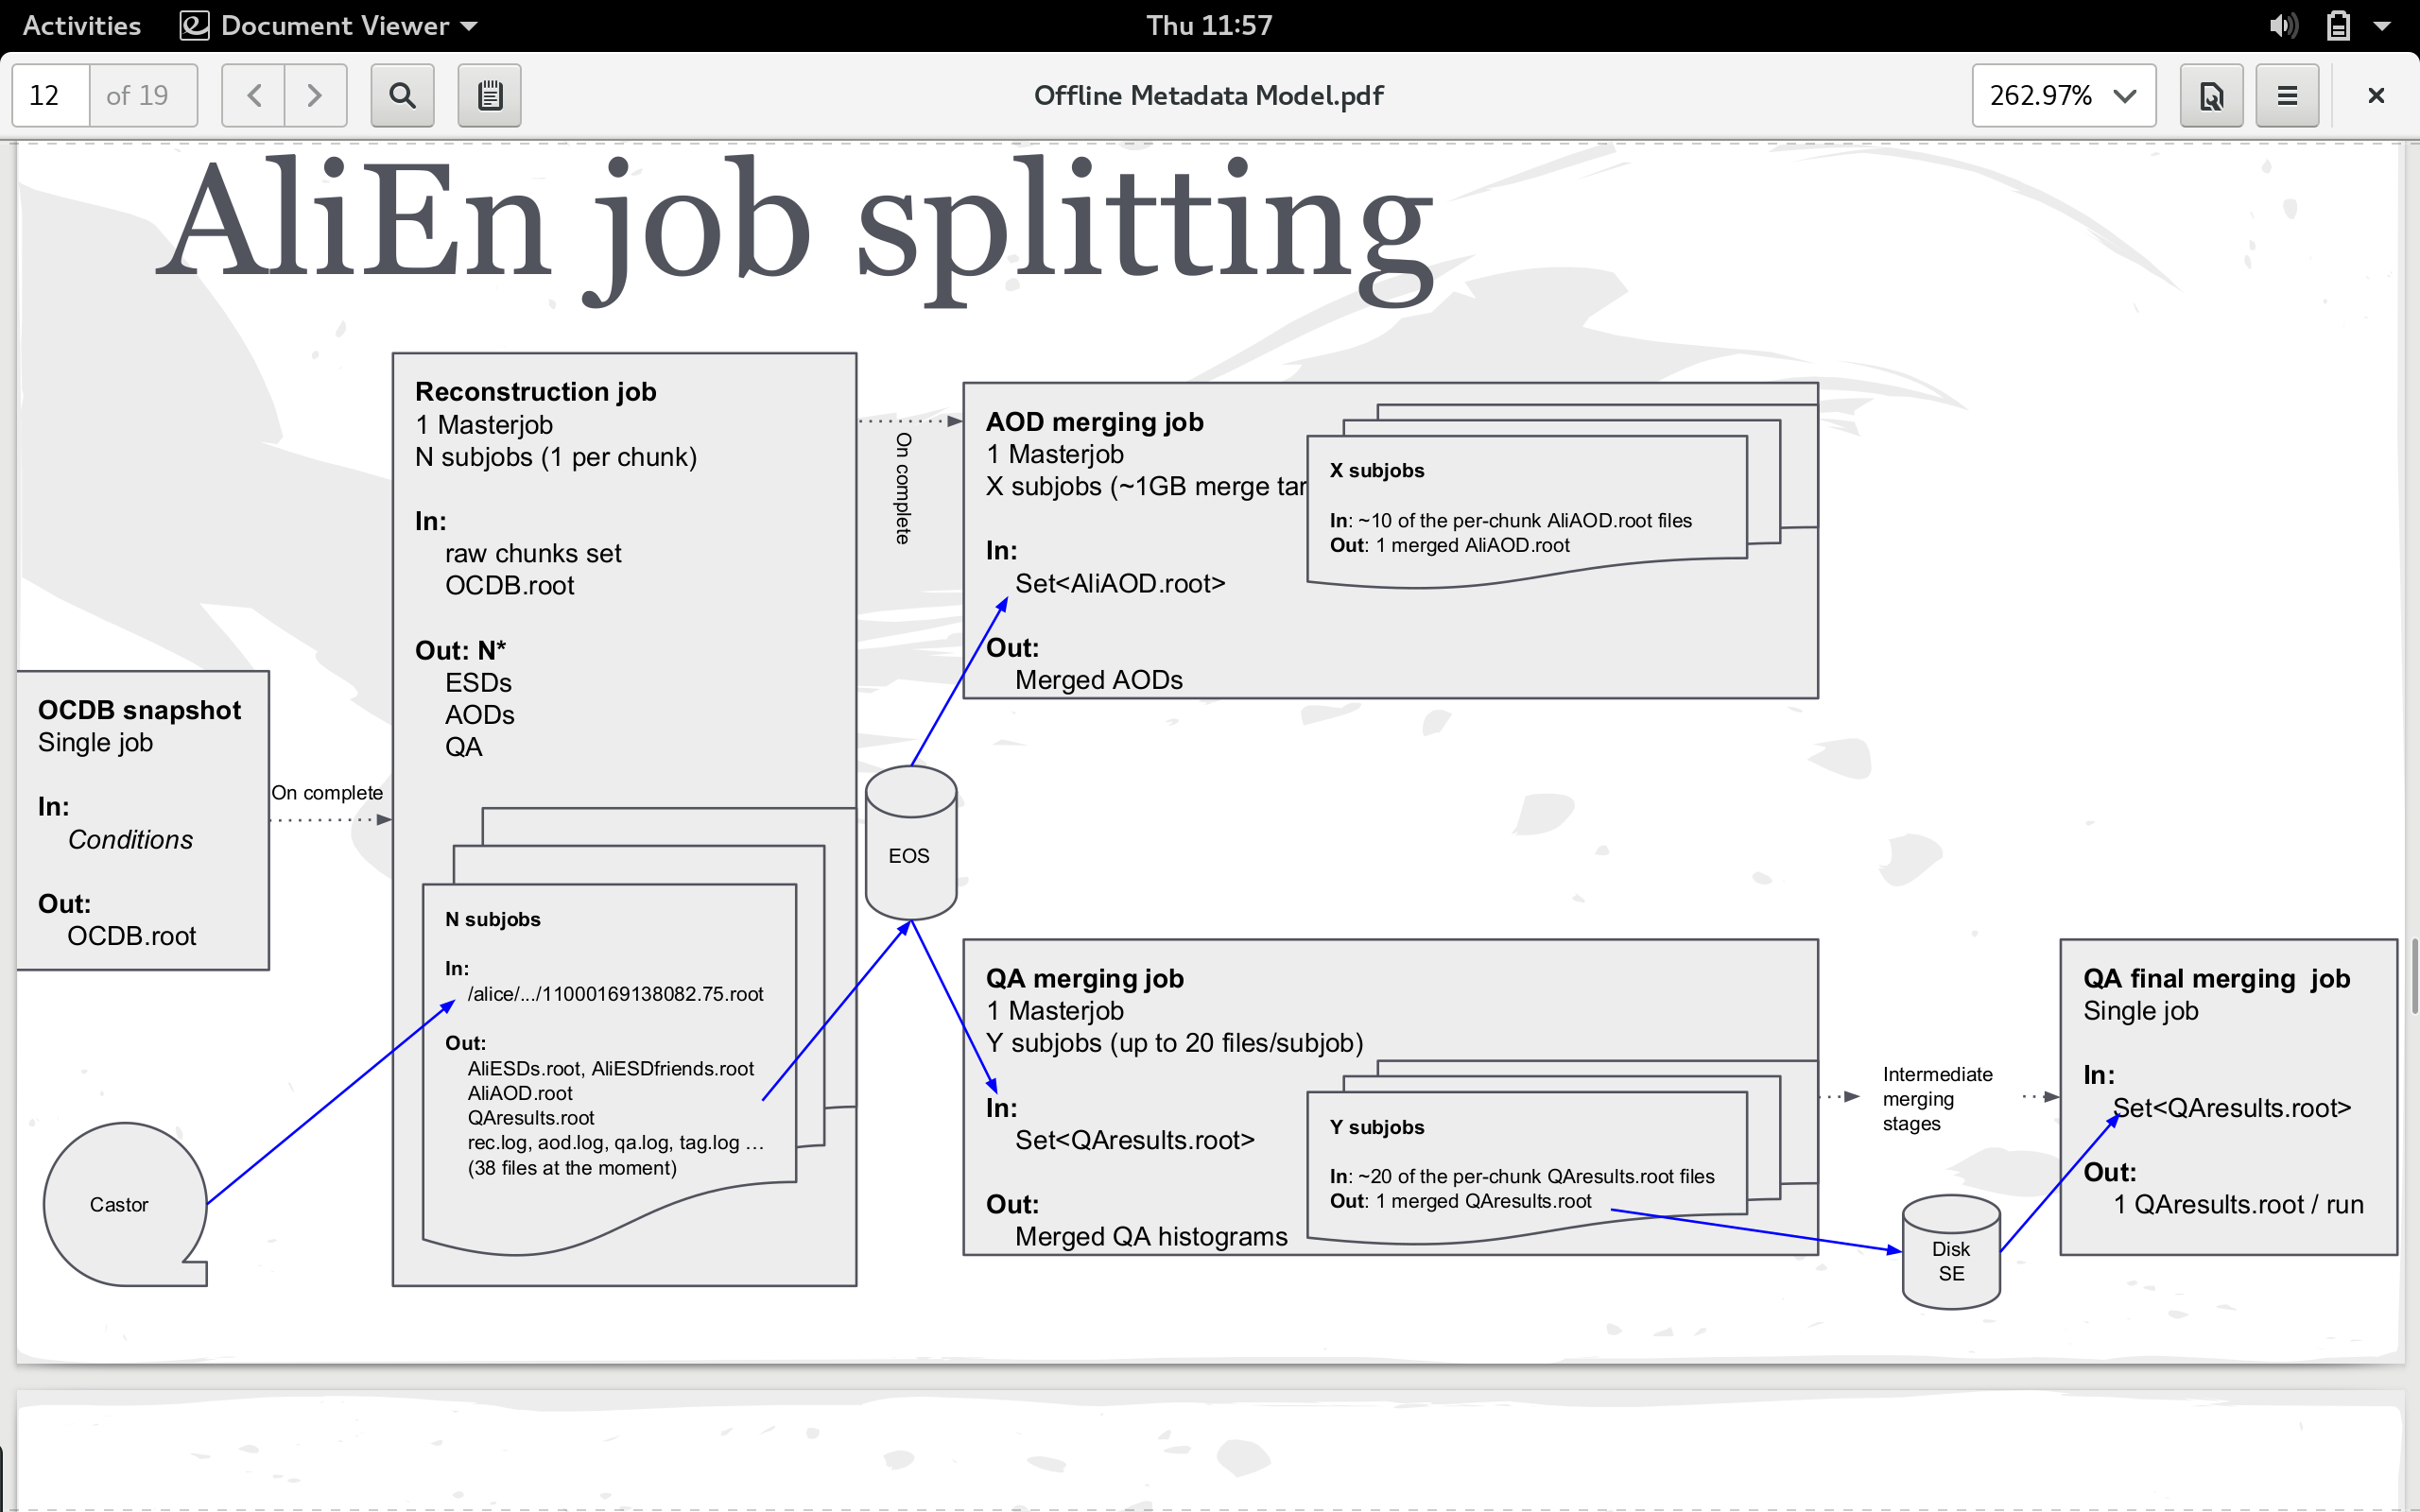
\includegraphics[scale=0.15]{./images/splitting_subjobs}
    \caption{Splitting jobs by AliEn}
    \label{fig:splitting_subjobs}
  \end{center}
\end{figure}

These jobs are executed independently. The used resources are monitored real time.

Subjobs are the finest granularity of processing. Each subjob has several parameters:
\begin{itemize}
  \item Software packages
  \item Environment, execution parameters
  \item Main executable and validation scripts
  \item Input set (data files, conditions, macros)
  \item Output set (results of the execution)
\end{itemize}
These execution logs are part of the output. This hard work as shown by some statistics. The number of jobs which run parallel  is 120,000. There is a turnover of 10 per second. Each second 200,000 entities are monitored and AliEn has to process 40,000 queries each second.

\subsubsection{RCT}
This data structure consists of:
\begin{itemize}
  \item Quality flags defined by detector experts
  \item Status code, color code, description
  \item Values associated to the same (run,pass) tuples
\end{itemize}
These parameters are set by QA experts of each detector group. Physic Work Groups (PWG) use this information to select specific and good runs for their analysis.

\subsubsection{Train}
A train is a considerable amount of jobs which all use the same data set. This is to reduce the I/O for all these jobs
The main metadata components of this data structure is:
\begin{itemize}
  \item Dataset (reference productions+file patterns+subset of runs)
  \item Software packages (one new tag daily)
  \item Participating wagons (tasks)
  \item Each gets the current event from the main loop
\end{itemize}
Each train is tested because its good practice and because the wagons are created by non-software engineers. There is a test machinery for each wagon and overall execution to prevent fatal errors and memory leaks and guarantee a reasonable CPU time. When a train is formed the LPM takes over for the submission, management, merging, notification of completion to end users

\subsubsection{JIRA production tickets}
In the JIRA produciton tickes running parameters are discussed. Also are quality and bugs tracked from the request.

\subsubsection{AliEn file catalog}
This is a set of input files as result of a `find` command. It results for instance in a number of OCDB files for a given run. There are 4 billion files in the namespace which amounts to 92 PB of data.

\subsubsection{Conclusion}
The new system should be linked to the file catalog which itself is outside the scope of the bookkeeping system development. It should be be an intermediate service. Concepts, procedures, work flow, metadata will stay the same.
 
\begin{table}[h]
\begin{center}
\begin{longtable}{ll}
    \hline
    ALICE & A Large Ion Collider Experiment\\
    \hline
    API & Application Programming Interface\\
    \hline
    DAQ & Data Acquisition subsystem \\
    \hline
    ID & Identity Document\\
    \hline
    IEEE & Institute of Electrical and Electronics Engineers\\
    \hline
     LHC  & Large Hydron Collider\\
     \hline
     $O^2$ & Online and Offline\\
     \hline
    \end{longtable}
      \caption{Acronyms}
  \label{tab:acronyms}
  \end{center}
  
\end{table}




\section{References}

\section{Overview}
This document is structured according to the IEEE standard 830-1998 Recommended Practice for Software Requirements Specifications.
